\documentclass[journal]{IEEEtran}

\ifCLASSINFOpdf
\usepackage[pdftex]{graphicx}
  % declare the path(s) where your graphic files are
\graphicspath{{../pdf/}{../jpeg/}}
  % and their extensions so you won't have to specify these with
  % every instance of \includegraphics
\DeclareGraphicsExtensions{.pdf,.jpeg,.png}
\else
  % or other class option (dvipsone, dvipdf, if not using dvips). graphicx
  % will default to the driver specified in the system graphics.cfg if no
  % driver is specified.
  % \usepackage[dvips]{graphicx}
  % declare the path(s) where your graphic files are
  % \graphicspath{{../eps/}}
  % and their extensions so you won't have to specify these with
  % every instance of \includegraphics
  % \DeclareGraphicsExtensions{.eps}
\fi

\usepackage[spanish]{babel}  % activa idioma español
\usepackage{titlesec}
\setcounter{secnumdepth}{5}



% *** MATH PACKAGES ***
\usepackage{amsmath}
\usepackage{amssymb}
\usepackage{amsthm}
\interdisplaylinepenalty=2500
% *** SPECIALIZED LIST PACKAGES ***
\usepackage{algorithmic}
% *** ALIGNMENT PACKAGES ***
\usepackage{array}
% *** SUBFIGURE PACKAGES ***
\ifCLASSOPTIONcompsoc
  \usepackage[caption=false,font=normalsize,labelfont=sf,textfont=sf]{subfig}
\else
  \usepackage[caption=false,font=footnotesize]{subfig}
\fi
% *** FLOAT PACKAGES ***
%\usepackage{fixltx2e}
%\usepackage{stfloats}
%\usepackage{dblfloatfix}

%\ifCLASSOPTIONcaptionsoff
%  \usepackage[nomarkers]{endfloat}
% \let\MYoriglatexcaption\caption
% \renewcommand{\caption}[2][\relax]{\MYoriglatexcaption[#2]{#2}}
%\fi
%\let\MYorigsubfloat\subfloat
%\renewcommand{\subfloat}[2][\relax]{\MYorigsubfloat[]{#2}}

% *** PDF, URL AND HYPERLINK PACKAGES ***
\usepackage{url}

\usepackage{float}
\usepackage{booktabs}

% correct bad hyphenation here
\hyphenation{op-tical net-works semi-conduc-tor}
\hyphenation{maxi-mizar REINFORCE}

\newtheorem{definition}{Definición}
\newtheorem{theorem}{Teorema}
\newtheorem{lemma}{Lema}
\newtheorem{proposition}{Proposición}

% Corolarios
\newtheorem{corollary}{Corolario}

% Subparagraph command
% \newcommand{\subparagraph}[1]{\vspace{1em}\noindent\textbf{#1.}}

\begin{document}
%
% paper title
% Titles are generally capitalized except for words such as a, an, and, as,
% at, but, by, for, in, nor, of, on, or, the, to and up, which are usually
% not capitalized unless they are the first or last word of the title.
% Linebreaks \\ can be used within to get better formatting as desired.
% Do not put math or special symbols in the title.
\title{Segmentación de Imágenes SEM mediante AutoML: \\
       Comparación de Estrategias de Segmentación}
%
%
% author names and IEEE memberships
% note positions of commas and nonbreaking spaces ( ~ ) LaTeX will not break
% a structure at a ~ so this keeps an author's name from being broken across
% two lines.
% use \thanks{} to gain access to the first footnote area
% a separate \thanks must be used for each paragraph as LaTeX2e's \thanks
% was not built to handle multiple paragraphs
%

\author{
    Darío Hernández Cubilla, 
    Diego Manuel Viera Martínez, 
    Francisco Préstamo Bernárdez, 
    Jossué Arteche Muñoz, 
    Luis Alejandro Arteaga Morales, 
    Mauricio Sunde Jimenez, 
    Pablo Gómez Vidal
    }


% make the title area
\maketitle
% As a general rule, do not put math, special symbols or citations
% in the abstract or keywords.
% \begin{abstract}
% The abstract goes here.
% \end{abstract}

% Note that keywords are not normally used for peerreview papers.
% \begin{IEEEkeywords}
% IEEE, IEEEtran, journal, \LaTeX, paper, template.
% end{IEEEkeywords}

\begin{abstract}
Se presenta un enfoque de aprendizaje automático para la detección de zonas frágiles y dúctiles en imágenes obtenidas mediante microscopía electrónica de barrido. El estudio compara modelos del estado del arte basados en transformers con estrategias de segmentación propuestas, integradas en un framework AutoML. La selección del modelo se realiza a partir de métricas de desempeño relevantes, considerando explícitamente las limitaciones computacionales del entorno de ejecución. Los resultados muestran la viabilidad del enfoque bajo recursos restringidos y evidencian el impacto del uso de aumentación de datos y transferencia de aprendizaje en la calidad de la segmentación.
\end{abstract}

\section{Introducción}
La caracterización de los mecanismos de fractura en materiales es un problema central en la ciencia e ingeniería de materiales, debido a su impacto directo en la evaluación del desempeño mecánico y la confiabilidad estructural. En particular, la identificación de zonas asociadas a comportamientos frágiles y dúctiles a partir de microestructuras proporciona información clave para el análisis del fallo y el diseño de materiales.

Las imágenes obtenidas mediante microscopía electrónica de barrido (SEM) constituyen una de las principales herramientas para el estudio de superficies de fractura y microestructuras. No obstante, el análisis tradicional de este tipo de imágenes se basa en inspección visual experta, lo cual introduce subjetividad, limita la reproducibilidad de los resultados y dificulta su aplicación a grandes volúmenes de datos.

En este contexto, las técnicas de aprendizaje automático y, en particular, los modelos de visión por computador han mostrado un potencial significativo para automatizar tareas de clasificación y segmentación en imágenes complejas. Recientemente, modelos basados en transformers, como Vision Transformer (ViT) y Swin Transformer, han alcanzado resultados destacados en diversas tareas de análisis de imágenes, posicionándose como referentes del estado del arte. Sin embargo, su aplicación práctica suele estar condicionada por la disponibilidad de datos anotados y recursos computacionales elevados.

Estas limitaciones motivan la exploración de estrategias alternativas que permitan aprovechar modelos de alto desempeño bajo restricciones de cómputo y datos. En este trabajo se consideran tanto modelos del estado del arte como enfoques propuestos basados en la descomposición espacial de la imagen y el uso de clasificadores preentrenados, con el objetivo de transferir conocimiento desde tareas de clasificación hacia problemas de segmentación.

Adicionalmente, se adopta un enfoque AutoML para automatizar la selección de modelos y el ajuste de hiperparámetros, empleando metaheurísticas y considerando explícitamente las restricciones impuestas por un entorno de cómputo limitado. El objetivo de este estudio es evaluar la viabilidad y el desempeño de estas estrategias para la detección de zonas frágiles y dúctiles en imágenes SEM, comparando modelos del estado del arte con enfoques alternativos bajo condiciones realistas de entrenamiento y evaluación.

% \section{Estado del arte}
% segmentacion
% clasificacion
% data augmentation
% evaluation

\section{Metodología basada en AutoML}
La resolución del problema de segmentación se abordó mediante un enfoque de AutoML diseñado específicamente para garantizar modularidad, reproducibilidad y comparabilidad sistemática entre distintas configuraciones experimentales. La metodología no se limita a la automatización del entrenamiento, sino que establece una arquitectura formal que define claramente cada etapa del flujo de datos y permite intercambiar componentes de manera controlada.

Arquitectura general del pipeline

El núcleo metodológico se basa en un pipeline lineal de procesamiento, en el cual los datos fluyen secuencialmente a través de nodos bien definidos. Este pipeline sigue el esquema general:

\begin{equation}
    \begin{aligned}
        \text{Dataset inicial} & \rightarrow \text{Nodo de aumentación} \rightarrow \text{Nodo de modelo} \\ 
        &\rightarrow \text{Nodo de evaluación} \rightarrow \text{Resultados finales}
    \end{aligned}
\end{equation}

Cada etapa del pipeline encapsula una responsabilidad única y explícita, evitando dependencias implícitas y facilitando el análisis aislado del impacto de cada decisión metodológica. La coordinación de este flujo está a cargo de una clase orquestadora central, denominada \emph{AutoML}, cuya función es estrictamente organizativa.

El diseño del framework se fundamenta en el uso extensivo de interfaces abstractas. Todas las etapas del pipeline implementan contratos formales definidos a nivel de interfaz, lo que permite desacoplar completamente la lógica de alto nivel de las implementaciones concretas. Este enfoque garantiza que diferentes estrategias —por ejemplo, distintos esquemas de validación o arquitecturas de red— puedan sustituirse sin alterar la estructura global del sistema.

La metodología adopta el principio de composición: la clase \emph{AutoML} no implementa lógica de entrenamiento, aumentación ni evaluación, sino que recibe instancias de nodos que cumplen interfaces predefinidas y las ejecuta en el orden correcto. Esto resulta en un núcleo extremadamente estable y fácil de auditar desde el punto de vista metodológico.

\subsection{Nodo de aumentación y partición de datos}
El primer componente del pipeline es el nodo de aumentación de datos, responsable de transformar el dataset original y generar las particiones de entrenamiento y validación. Este nodo recibe el dataset completo y produce una lista de pares 
$(D_{train},D_{val})$ lo que permite soportar tanto divisiones simples como esquemas de validación cruzada k-fold.

Desde el punto de vista metodológico, esta decisión es clave: todas las transformaciones de datos y estrategias de partición quedan formalizadas en un único punto del pipeline, evitando fugas de información y asegurando que todos los modelos evaluados operen bajo condiciones comparables.

\subsection{Nodo de modelo}
El nodo de modelo constituye el núcleo computacional del sistema. Para cada par de datasets generado por el nodo de aumentación, este componente entrena una instancia del modelo especificado y posteriormente genera predicciones sobre el conjunto de validación. El resultado de esta etapa es una colección estructurada de pares de máscaras predichas y reales, organizada por pliegue cuando corresponde.

Cada arquitectura se encapsula en una implementación concreta de este nodo, manteniendo la misma interfaz externa. Esto permite comparar modelos de distinta naturaleza bajo un marco experimental idéntico, aislando el efecto de la arquitectura del resto del pipeline.

\subsection{Nodo de evaluación}
El nodo de evaluación recibe exclusivamente las predicciones y las máscaras reales producidas por el nodo de modelo. Su responsabilidad es calcular las métricas de desempeño de forma agregada y consistente. Internamente, este nodo delega el cálculo a evaluadores individuales, cada uno asociado a una métrica específica.

Desde el punto de vista metodológico, este desacoplamiento garantiza que las métricas no influyan en el proceso de entrenamiento ni en la generación de predicciones, evitando sesgos y permitiendo incorporar nuevas métricas sin modificar etapas previas del pipeline.

\subsection{Orquestación y ejecución automática}
La clase \emph{AutoML} actúa como el punto único de ejecución del experimento. Su método principal ejecuta secuencialmente los nodos de aumentación, modelo y evaluación, y retorna un conjunto final de métricas. Este diseño minimalista reduce la complejidad cognitiva del sistema y asegura que el flujo experimental sea explícito y reproducible.

La automatización se logra mediante la ejecución repetida del pipeline con distintas combinaciones de nodos y configuraciones. De este modo, el proceso de selección de modelos e hiperparámetros se formaliza como una exploración sistemática del espacio de configuraciones, donde el criterio de selección se basa exclusivamente en las métricas producidas por el nodo evaluador.

La construcción concreta de los nodos no se realiza directamente en los scripts experimentales, sino mediante funciones de configuración ubicadas en un módulo dedicado. Este enfoque separa claramente la definición del experimento de la lógica interna del framework, mejorando la legibilidad, reduciendo errores de configuración y facilitando la reproducibilidad de los resultados.

Esta metodología basada en \emph{AutoML} establece una base sólida y extensible para todo el desarrollo posterior, dentro de un marco experimental unificado y controlado.

\section{Descripción del dataset}
% - División train/test
% - Origen de las imágenes SEM
% - Dimensiones (512x512)
% - Clases de segmentación (frágil, dúctil, mixto)
% - Distribución de clases
A continuación se proporciona información sobre los datasets utilizados.
\subsection{Dataset de segmentación}

El dataset principal utilizado para la tarea de segmentación está compuesto por 94 imágenes obtenidas mediante microscopía electrónica de barrido (SEM) utilizando un microscopio Vega 3 Scan. Cada imagen cuenta con su correspondiente máscara de segmentación a nivel de píxel.

Las máscaras consideran exclusivamente dos clases mutuamente excluyentes: material frágil y material dúctil. A nivel global, el conjunto presenta un desbalance significativo entre clases, con 73 imágenes predominantemente dúctiles y 21 imágenes predominantemente frágiles. Esta distribución refleja la naturaleza del material analizado y constituye un desafío adicional.

Las imágenes originales presentan tamaños variables, lo cual motivó la adopción de un preprocesamiento de redimensionamiento a una resolución fija de $512 \times 512$ píxeles para los modelos basados en transformers y para el análisis estadístico espacial.

Con el objetivo de caracterizar la distribución espacial de las clases, se construyó el mapa de calor de la Figura~\ref{fig:heatmap_ductil} agregando las máscaras redimensionadas. Dado que las clases son excluyentes, el mapa de calor representa únicamente la frecuencia de la clase dúctil. Este análisis permitió identificar regiones con mayor recurrencia de comportamiento dúctil, así como zonas donde la presencia de material frágil es más probable, aportando una visión global de la estructura espacial del dataset.

\begin{figure}[t]
    \centering
    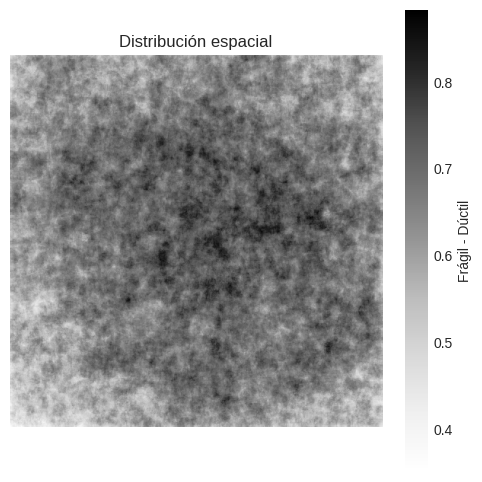
\includegraphics[width=\linewidth]{heatmap.png}
    \caption{Mapa de calor de la distribución espacial de las clases dúctil y frágil, obtenido a partir de la superposición de las máscaras de segmentación redimensionadas a $512 \times 512$ píxeles.}
    \label{fig:heatmap_ductil}
\end{figure}


\subsection{Dataset externo de clasificación}

Para las tareas de clasificación, en particular aquellas asociadas a los enfoques basados en Quadtree y Sliding Window, se utilizó un dataset externo independiente del conjunto de segmentación. Este dataset fue empleado para entrenar los clasificadores auxiliares encargados de etiquetar regiones completas de imagen.

El conjunto de datos corresponde al dataset de imágenes SEM publicado por Campari~\cite{campari_2025_15510590}, el cual contiene imágenes de microscopía electrónica anotadas a nivel de imagen para tareas de clasificación. El uso de este dataset permitió desacoplar el entrenamiento de los clasificadores del proceso de segmentación, habilitando estrategias de transferencia de aprendizaje desde clasificación hacia segmentación regional.

Cabe destacar que este dataset externo no fue utilizado en ninguna etapa del entrenamiento de los modelos de segmentación directa, ni en la construcción del conjunto de prueba, garantizando así la independencia entre las fuentes de datos.


\section{Estrategias de Segmentación}
La segmentación de zonas frágiles y dúctiles se aborda mediante un conjunto de estrategias complementarias que responden a distintos niveles de complejidad y granularidad en la representación de la imagen. En primer lugar, se consideran arquitecturas basadas en Vision Transformers y Swin Transformers, seleccionadas por su capacidad para modelar dependencias espaciales de largo alcance y por su consolidación como enfoques de referencia en tareas de segmentación densa. Estos modelos permiten aprender representaciones globales y jerárquicas directamente a partir de la imagen completa, proporcionando una base sólida para la identificación precisa de regiones con comportamiento mecánico diferenciado.

De forma complementaria, se exploran estrategias de segmentación indirecta que reutilizan conocimiento previamente adquirido en tareas de clasificación. En este enfoque, la información semántica extraída por modelos entrenados para discriminar regiones frágiles y dúctiles se emplea como guía para definir esquemas de segmentación basados en particiones espaciales adaptativas. En particular, se consideran métodos que descomponen la imagen en regiones locales cuya resolución y extensión se ajustan dinámicamente en función de la complejidad visual y la confianza de la clasificación, permitiendo una transición controlada entre análisis global y local.

Este planteamiento unifica modelos de segmentación directa y estrategias guiadas por clasificación bajo un mismo marco conceptual, facilitando la comparación entre enfoques de distinta naturaleza y sentando las bases para la incorporación progresiva de métodos alternativos de particionado espacial en subsecciones posteriores.

\subsection{Vision Transformer (ViT)}
% - Arquitectura general
% - División en patches
% - Mecanismo de atención
% - Adaptación para segmentación semántica
% - Hiperparámetros utilizados

La estrategia de segmentación basada en \emph{Vision Transformer} (ViT) se diseñó siguiendo un enfoque modular que separa explícitamente la definición arquitectónica del modelo del proceso de entrenamiento y evaluación. Esta decisión metodológica permite desacoplar los aspectos conceptuales del modelo de los detalles operativos, facilitando su integración en el framework de \emph{AutoML} y asegurando comparabilidad con otras estrategias de segmentación.

\subsubsection{Arquitectura encoder--decoder}

El modelo adopta una arquitectura de tipo \emph{encoder--decoder}, donde el encoder se basa en un Transformer y el decoder en una red neuronal convolucional. Esta combinación permite explotar la capacidad del mecanismo de autoatención para capturar dependencias globales, mientras que el decoder convolucional reconstruye la información espacial necesaria para una segmentación densa a nivel de píxel.

El encoder transforma la imagen de entrada en una secuencia de representaciones latentes mediante un proceso de partición en parches no solapados. Cada parche es proyectado a un espacio de alta dimensionalidad, generando una secuencia de \emph{embeddings} que reemplaza la representación basada en píxeles. Dado que los Transformers carecen de noción explícita de orden espacial, se incorporan codificaciones posicionales aprendibles, las cuales preservan la información relativa a la localización de cada parche en la imagen original.

Posteriormente, esta secuencia es procesada por múltiples capas de autoatención, donde cada parche puede intercambiar información con todos los demás. Este mecanismo permite construir representaciones con contexto global, capturando relaciones de largo alcance.

\subsubsection{Decoder convolucional y reconstrucción espacial}

La salida del encoder, expresada como una secuencia de vectores latentes, es reestructurada nuevamente en forma de mapa bidimensional de características. A partir de esta representación de baja resolución espacial, el decoder convolucional realiza una reconstrucción progresiva hasta alcanzar la resolución original de la imagen.

Este proceso se lleva a cabo mediante una serie de etapas de refinamiento y reescalado, en las cuales se combinan convoluciones para la extracción local de características con operaciones de interpolación para el aumento gradual de la resolución. En la etapa final, una proyección lineal por píxel permite obtener, para cada clase, un mapa de activación que representa la pertenencia de cada píxel a las distintas regiones de interés.

\subsubsection{Integración en el pipeline de AutoML}

La arquitectura ViT descrita se integra en el pipeline de AutoML mediante un componente que encapsula tanto el proceso de entrenamiento como la generación de predicciones. Este componente actúa como intermediario entre el modelo de segmentación y el resto del framework, garantizando que el ViT pueda ser tratado de manera homogénea junto con otras arquitecturas.

Durante el entrenamiento, se emplea un esquema supervisado estándar para segmentación multiclase, utilizando funciones de pérdida adecuadas para este tipo de problema y validación sobre datos no vistos para monitorear el desempeño. En la fase de inferencia, las salidas continuas del modelo son convertidas en máscaras discretas mediante una asignación por máxima activación, produciendo mapas de segmentación directamente comparables con las máscaras de referencia.

Esta estrategia combina la capacidad de los Vision Transformers para modelar contexto global con la precisión espacial de decodificadores convolucionales, resultando adecuada para problemas de segmentación.

\subsection{Swin Transformer}

El segmentador basado en \emph{Swin Transformer} se desarrolló siguiendo el mismo principio aplicado al modelo ViT: una separación estricta entre la arquitectura del modelo y la lógica de entrenamiento y evaluación. Esta coherencia de diseño garantiza modularidad, facilita la comparación experimental y permite integrar el modelo de manera transparente dentro del framework de AutoML.

\subsubsection{Arquitectura encoder--decoder}

Al igual que en el caso del ViT, el modelo adopta una arquitectura de tipo \emph{encoder--decoder}. Sin embargo, el encoder se basa en el Swin Transformer, una evolución de los Transformers para visión computacional que introduce propiedades jerárquicas y de localidad, tradicionalmente asociadas a las redes convolucionales.

El encoder genera representaciones jerárquicas a múltiples escalas espaciales. A partir de la imagen de entrada, el modelo construye progresivamente un conjunto de mapas de características con resoluciones decrecientes, lo que permite capturar información tanto local como global. Este enfoque multiescala resulta especialmente adecuado para tareas de segmentación, donde coexisten detalles finos y estructuras de mayor tamaño.

El mecanismo central del Swin Transformer es la autoatención restringida a ventanas locales, lo que reduce significativamente la complejidad computacional en comparación con la autoatención global. Para evitar la pérdida de información entre regiones disjuntas, estas ventanas se desplazan de manera alternada entre capas consecutivas, permitiendo que la información fluya entre distintas zonas de la imagen. De este modo, el modelo combina eficiencia computacional con una capacidad efectiva de modelar dependencias de largo alcance.

Adicionalmente, la arquitectura fue adaptada para operar sobre imágenes en escala de grises, lo que asegura compatibilidad con el tipo de datos empleado en este trabajo sin alterar los principios fundamentales del modelo.

\subsubsection{Adaptación de resolución y decoder compartido}

El encoder basado en Swin Transformer produce su representación final a una resolución espacial inferior a la utilizada por el decoder convolucional. Para resolver esta discrepancia, se introduce un módulo de adaptación intermedio que reescala las características extraídas por el encoder hasta la resolución esperada por el decoder.

Una vez ajustada la resolución, las características son procesadas por el mismo decoder convolucional utilizado en el modelo basado en ViT. Este decoder realiza una reconstrucción progresiva de la segmentación mediante etapas sucesivas de refinamiento y aumento de resolución, culminando en un mapa de segmentación denso a nivel de píxel. El uso de un decoder compartido evita la duplicación de componentes, mejora la mantenibilidad del sistema y asegura que las diferencias observadas en los resultados se deban principalmente al encoder y no a variaciones en la fase de reconstrucción.

\subsubsection{Entrenamiento, regularización y evaluación}

La integración del modelo Swin en el pipeline de AutoML se realiza a través de un componente que encapsula el proceso completo de entrenamiento y evaluación, manteniendo la misma interfaz que otros segmentadores. Esto garantiza la interoperabilidad dentro del framework y permite su comparación directa con enfoques alternativos.

Un aspecto distintivo de esta estrategia es la incorporación de un mecanismo de \emph{early stopping} durante el entrenamiento. Este mecanismo monitoriza el desempeño sobre el conjunto de validación y detiene el proceso de optimización cuando no se observan mejoras durante un número predefinido de iteraciones consecutivas. De este modo, se reduce el riesgo de sobreajuste y se selecciona automáticamente el estado del modelo con mejor capacidad de generalización.

En la fase de inferencia, el modelo genera mapas de activación multiclase que son transformados en máscaras de segmentación discretas mediante una asignación por máxima respuesta. Estas máscaras se utilizan posteriormente en el módulo de evaluación, asegurando consistencia con el resto de modelos analizados.

El segmentador basado en Swin Transformer combina eficiencia computacional, representación jerárquica multiescala y mecanismos de regularización explícitos, constituyendo una alternativa de alto nivel dentro del estado del arte para segmentación semántica en imágenes complejas.


\subsection{Descomposición quadtree}

El enfoque de segmentación basado en quadtree difiere de manera fundamental de los modelos neuronales de tipo extremo a extremo. En lugar de aprender directamente una correspondencia píxel a píxel, este método se formula como un algoritmo recursivo de tipo \emph{divide y vencerás}, que combina un modelo de clasificación independiente con una estrategia adaptativa de partición espacial. Esta aproximación permite razonar sobre regiones completas de la imagen y ajustar dinámicamente el nivel de detalle de la segmentación en función de la complejidad local.

\subsubsection{Principio de divide y vencerás mediante quadtree}

El algoritmo opera de manera recursiva sobre regiones rectangulares de la imagen. Inicialmente, la imagen completa se considera como una única región. Para cada región analizada, se consulta a un clasificador externo con el fin de estimar la clase predominante y un nivel de confianza asociado a dicha predicción.

Si la confianza supera un umbral predefinido, se asume que la región es suficientemente homogénea y se asigna la clase predicha a todos los píxeles que la componen. En caso contrario, el algoritmo interpreta que la región contiene información heterogénea o ambigua y procede a subdividirla en cuatro cuadrantes de igual tamaño. Este proceso se repite de forma independiente para cada subregión.

La recursión se detiene cuando se cumple alguna de las siguientes condiciones: la confianza del clasificador es suficiente, la región alcanza un tamaño mínimo que impide una subdivisión significativa, o se llega a una profundidad máxima de recursión. Como resultado, el método genera regiones extensas y uniformes en zonas simples de la imagen, y particiones más finas en áreas con mayor complejidad estructural.

\subsubsection{Separación entre segmentación y clasificación}

Un rasgo central de este enfoque es la separación explícita entre la lógica de segmentación y el modelo de clasificación utilizado para tomar decisiones locales. El algoritmo quadtree se limita a gestionar la recursión y la asignación espacial de etiquetas, mientras que el clasificador actúa como un componente intercambiable encargado de evaluar regiones de la imagen.

Esta separación permite desacoplar completamente la estrategia de partición del método concreto de clasificación empleado. En consecuencia, es posible evaluar distintos clasificadores bajo un mismo esquema de segmentación sin modificar el algoritmo quadtree, lo que aporta flexibilidad experimental y facilita el análisis comparativo de modelos.

\subsubsection{Proceso de ajuste de parámetros mediante metaheurísticas}

A diferencia de los modelos neuronales clásicos, el proceso de entrenamiento de este segmentador no se basa en retropropagación de gradientes. En su lugar, el ajuste se centra en la optimización de los hiperparámetros que controlan el comportamiento del algoritmo recursivo, tales como el umbral de confianza, el tamaño mínimo de región y la profundidad máxima de subdivisión.

Este ajuste se plantea como un problema de optimización global y se resuelve mediante una metaheurística de recocido simulado (\emph{simulated annealing}). El procedimiento explora el espacio de hiperparámetros evaluando configuraciones candidatas sobre un conjunto de validación, aceptando tanto mejoras directas como, de manera probabilística, configuraciones subóptimas en etapas tempranas de la búsqueda. Este mecanismo permite escapar de óptimos locales y favorece una exploración más amplia del espacio de soluciones.

Al finalizar el proceso, el algoritmo conserva la configuración de hiperparámetros que produjo el mejor desempeño global, la cual se fija para la generación de resultados finales.

\subsubsection{Generación y evaluación de las segmentaciones}

Durante la fase de evaluación, el algoritmo se aplica de manera independiente a cada imagen del conjunto de datos. A partir de una máscara inicialmente vacía, el proceso recursivo va asignando etiquetas a las distintas regiones según las decisiones tomadas en cada nivel de la jerarquía quadtree. El resultado final es una máscara de segmentación completa, construida de forma adaptativa en función de la complejidad local de la imagen.

Las máscaras predichas se comparan posteriormente con las máscaras de referencia mediante las métricas definidas en el framework de evaluación, lo que permite analizar cuantitativamente el desempeño del método y contrastarlo con los enfoques basados en redes neuronales profundas.


\section{Modelos de clasificación para segmentación}
En esta sección se describen los modelos de clasificación empleados como componentes fundamentales de las estrategias de segmentación guiada basadas en particionado espacial. A diferencia de los enfoques de segmentación directa, estos métodos delegan la toma de decisiones semánticas a clasificadores entrenados para discriminar entre zonas frágiles y dúctiles, cuya salida se utiliza posteriormente para construir máscaras de segmentación a distintas escalas.

El objetivo de esta sección es caracterizar los clasificadores utilizados, independientemente del esquema de particionado específico en el que se integran. De este modo, se separa explícitamente el análisis del modelo de clasificación del mecanismo geométrico de segmentación, permitiendo evaluar de forma aislada el impacto de la arquitectura del clasificador en el desempeño final del sistema. Las subsecciones siguientes presentan los distintos modelos considerados.

\subsection{Clasificador CNN}

El clasificador basado en Redes Neuronales Convolucionales (CNN) fue diseñado 
para clasificar regiones de tamaño variable extraídas por el algoritmo Quadtree.

% \subparagraph{Arquitectura General}

La arquitectura sigue un patrón de extracción de características seguido de 
clasificación:

\begin{equation}
    \begin{aligned}
        \text{Entrada} &\rightarrow \text{Bloques Conv.} \rightarrow 
        \text{Pooling Global} \\
        &\rightarrow \text{Clasificador} \rightarrow \text{Softmax}
    \end{aligned}
\end{equation}

% \subparagraph{Bloques Convolucionales}

Cada bloque convolucional aplica la siguiente secuencia:

\begin{enumerate}
    \item Convolución 3×3 con padding=1
    \item Batch Normalization
    \item Activación ReLU
    \item Convolución 3×3 con padding=1
    \item Batch Normalization
    \item Activación ReLU
    \item Max Pooling 2×2 con stride=2
\end{enumerate}

Se usa un kernel de $3 \times 3$ porque es el tamaño mínimo que captura información 
espacial (arriba, abajo, izquierda, derecha y diagonales). Al apilar múltiples 
capas con kernels pequeños se obtiene un campo receptivo grande con menos 
parámetros que usando un kernel grande directamente.

El padding de $1$ píxel mantiene las dimensiones espaciales constantes después 
de cada convolución, lo que simplifica el diseño de la red.

Batch Normalization se incluye para acelerar el entrenamiento y estabilizar 
los gradientes, permitiendo usar tasas de aprendizaje más altas.

Se usan dos convoluciones por bloque antes del pooling para aumentar la 
capacidad de la red sin reducir las dimensiones espaciales prematuramente.

% \subparagraph{Número Configurable de Bloques}

El parámetro \texttt{num\_blocks} controla la profundidad de la red. Como cada 
bloque reduce las dimensiones a la mitad mediante Max Pooling, el tamaño mínimo 
de entrada es $2^{n} \times 2^{n}$ píxeles, donde $n$ es el número de bloques.

\begin{table}[h]
\centering
\caption{Relación entre número de bloques y tamaño mínimo de entrada}
\begin{tabular}{ccc}
\toprule
\texttt{num\_blocks} & Tamaño mínimo & Canales finales \\
\midrule
2 & 4×4 & 64 \\
3 & 8×8 & 128 \\
4 & 16×16 & 256 \\
5 & 32×32 & 512 \\
\bottomrule
\end{tabular}
\label{tab:cnn_blocks}
\end{table}

El valor por defecto es 3 bloques, lo que permite clasificar regiones de 8×8 
píxeles. Este tamaño fue elegido porque el Quadtree puede subdividir hasta 
regiones pequeñas, y 8×8 se consideró suficiente para contener información visual 
distinguible mientras permite segmentación detallada.

% \subparagraph{Progresión de Filtros}

El número de filtros se duplica en cada bloque, comenzando desde 32:

\begin{equation}
    \text{filtros en bloque } i = 32 \times 2^{i-1}
\end{equation}

Esta progresión compensa la reducción de dimensiones espaciales: a medida que 
la imagen se hace más pequeña, se aumentan los canales para mantener la 
capacidad de representación.

% \subparagraph{Adaptive Average Pooling}

Antes de la clasificación se aplica \texttt{AdaptiveAvgPool2d((1,1))}, que 
reduce cualquier tamaño espacial a 1×1 calculando el promedio de cada canal.

Esta capa permite que la red acepte entradas de cualquier tamaño (siempre que 
cumplan el mínimo). Sin importar si la entrada es 8×8 o 256×256, la salida 
siempre es un vector de tamaño fijo que puede procesarse por las capas 
densas.

% \subparagraph{Cabeza de Clasificación}

La cabeza de clasificación consiste en:

\begin{enumerate}
    \item Aplanamiento del tensor
    \item Dropout (50\%)
    \item Capa densa con reducción a 1/4 de los canales
    \item Activación ReLU
    \item Dropout (25\%)
    \item Capa densa final a 3 clases
\end{enumerate}

El Dropout previene sobreajuste, que es una preocupación con datasets pequeños 
de imágenes SEM. La capa intermedia reduce la dimensionalidad gradualmente 
antes de la clasificación final.

% \subparagraph{Salida}

La red produce probabilidades mediante Softmax, donde la probabilidad más alta 
indica la clase predicha y su valor representa la confianza. Esta confianza es 
usada por el Quadtree para decidir si subdividir la región o aceptar la 
clasificación.

% \subparagraph{Entrenamiento}

El entrenamiento usa Cross-Entropy Loss y el optimizador Adam. Las imágenes se 
agrupan por tamaño para formar batches, ya que las regiones del Quadtree tienen 
dimensiones variables y solo se pueden apilar en un tensor imágenes del mismo 
tamaño.

\subsection{Clasificador ViT}

El clasificador basado en Vision Transformer se utiliza como un componente auxiliar dentro del esquema de segmentación jerárquica, con el objetivo de asignar una única etiqueta a regiones completas de la imagen. A diferencia de los modelos de segmentación, este enfoque no opera a nivel de píxel, sino que produce una predicción global acompañada de una medida de confianza, la cual resulta fundamental para guiar las decisiones del algoritmo quadtree.

\subsubsection{Arquitectura del clasificador}

La arquitectura adoptada corresponde a un Vision Transformer estándar para tareas de clasificación de imágenes, cuyo elemento distintivo es el uso de un token de clasificación. La imagen de entrada se divide inicialmente en parches de tamaño fijo, los cuales son proyectados a un espacio de características de alta dimensión mediante un proceso de incrustación. A estas representaciones se les añade información posicional aprendible, permitiendo al modelo preservar las relaciones espaciales entre los distintos parches.

Sobre esta secuencia de representaciones se introduce un token de clasificación, el cual no está asociado a ninguna región específica de la imagen. Este token se antepone a la secuencia de parches y participa activamente en los mecanismos de autoatención del transformer. A lo largo de las capas del encoder, el token de clasificación actúa como un agregador de información global, concentrando en una única representación los patrones más relevantes presentes en la imagen completa.

Finalizado el procesamiento por el transformer, se descartan las representaciones asociadas a los parches y se conserva únicamente el vector correspondiente al token de clasificación. Este vector se proyecta mediante una cabeza de clasificación hacia el espacio de clases, generando puntuaciones que se transforman en probabilidades normalizadas. Estas probabilidades permiten obtener tanto la etiqueta predicha como una estimación explícita de la confianza del modelo.

\subsubsection{Uso del clasificador en regiones de tamaño arbitrario}

Dado que el clasificador se emplea para evaluar regiones de distinto tamaño dentro del esquema quadtree, resulta necesario un preprocesamiento que garantice la compatibilidad con la entrada de tamaño fijo requerida por el Vision Transformer. Cada región extraída de la imagen original se normaliza en formato y número de canales, y posteriormente se redimensiona mediante interpolación a la resolución esperada por el modelo.

Este procedimiento permite aplicar un clasificador entrenado sobre imágenes completas a subregiones arbitrarias, manteniendo la coherencia de las predicciones y asegurando una integración transparente con el algoritmo de segmentación jerárquica.

\subsubsection{Entrenamiento y rol dentro del framework}

El clasificador puede entrenarse de manera independiente sobre conjuntos de datos externos de clasificación, utilizando un esquema supervisado estándar. Una vez finalizado el entrenamiento, el modelo se emplea principalmente en modo de inferencia, proporcionando predicciones rápidas y consistentes durante la ejecución del algoritmo quadtree.

Dentro del framework AutoML, este clasificador actúa como un componente intercambiable, lo que permite evaluar distintas arquitecturas de clasificación bajo el mismo esquema de segmentación. De este modo, el análisis se centra en estudiar cómo la capacidad discriminativa del clasificador influye en la calidad final de la segmentación basada en descomposición jerárquica.



\section{Pipeline de Aumentación de Datos}
Se implementó un conjunto completo de técnicas de aumentación de datos con el objetivo de incrementar la diversidad del dataset y mejorar la generalización de los modelos. La estrategia combinó transformaciones geométricas, fotométricas y específicas para SEM, aplicadas de manera secuencial y probabilística según un pipeline de aumentación.

\subsubsection{Aumentaciones Geométricas}
% - Rotación, volteo, escala, traslación, recorte
% - Aplicación simultánea a imagen y máscara
Afectan tanto a imágenes como a máscaras, manteniendo la alineación espacial:

\begin{itemize}
    \item Rotación: Rota la imagen y la máscara dentro de un rango definido, simulando diferentes orientaciones de la muestra.
    \item Volteo: Invierte horizontal o verticalmente.
    \item Escalado: Realiza zoom in/out manteniendo el tamaño original.
    \item Traslación: Desplaza la imagen y máscara horizontal y/o verticalmente.
    \item Recorte aleatorio: Extrae subregiones aleatorias, redimensionadas al tamaño original.
\end{itemize}

Estas transformaciones permiten al modelo generalizar a variaciones espaciales de la muestra.

\subsubsection{Aumentaciones Fotométricas}
% - Brillo, contraste, ruido gaussiano, desenfoque, gamma
% - Aplicación solo a imagen (no a máscara)

Modifican únicamente las imágenes, simulando variaciones en iluminación y ruido, sin afectar las máscaras:

\begin{itemize}
    \item Brillo.
    \item Contraste.
    \item Corrección gamma.
    \item Ruido gaussiano.
    \item Desenfoque gaussiano.
\end{itemize}

Estas técnicas permiten al modelo aprender invariancia frente a condiciones de adquisición o ruido instrumental.

\subsubsection{Aumentaciones Específicas para SEM}
Diseñadas para capturar artefactos y características típicas de imágenes SEM:

\begin{itemize}
    \item Deformación elástica (ElasticDeformationAugmentator): Simula variaciones naturales en texturas de roca o deformaciones durante la adquisición.
    \item Ecualización adaptativa de histograma (AdaptiveHistogramEqualizationAugmentator): Mejora contraste local mediante CLAHE.
    \item Artefactos de carga: Añade manchas típicas de muestras no conductivas.
    \item Ruido de líneas de escaneo (ScanLineNoiseAugmentator): Simula líneas de escaneo o barrido que aparecen en SEM.
\end{itemize}

Estas técnicas aumentan la robustez del modelo frente a artefactos específicos de la microscopía electrónica.

\subsubsection{Composición de Aumentaciones}
% - Secuencial, selección aleatoria, aplicación probabilística
% - Estrategias de combinación utilizadas
Se implementaron métodos compuestos que permiten combinar varias aumentaciones para crear un pipeline complejo y controlado:

\begin{itemize}
    \item Secuencial: Aplica múltiples aumentaciones de manera secuencial.
    \item Aplicación probabilistica: Aplica una aumentación con una probabilidad determinada, introduciendo variabilidad controlada.
    \item Selección aleatoria: Elige una aumentación de un conjunto con probabilidades ponderadas.
\end{itemize}

Estas estrategias permiten generar un dataset enriquecido sin comprometer la coherencia entre imágenes y máscaras.

\subsection{Métricas de Evaluación}
La evaluación del desempeño de los modelos de segmentación se diseñó de forma modular y extensible, permitiendo calcular múltiples métricas a partir de una representación común de las predicciones y las máscaras de referencia. Todo el proceso es coordinado por un nodo evaluador central (\emph{EvaluatorNode}), cuyo objetivo es desacoplar la generación de predicciones del cálculo de métricas, facilitando comparaciones consistentes entre modelos y configuraciones experimentales.

Para cada imagen del conjunto de validación, el modelo de segmentación genera una máscara predicha, la cual se empareja con su máscara real correspondiente. Este proceso produce una colección de pares 
$(\hat M,M)$, denominada \emph{MaskPairs}. En escenarios con validación cruzada k-fold, estas colecciones se agrupan por pliegue, resultando en una estructura del tipo lista de listas; en el caso simple de train/validation split, existe un único conjunto de pares.

Esta estructura es la entrada principal del \emph{EvaluatorNode}, que no calcula métricas directamente, sino que delega el cómputo a evaluadores especializados. Cada evaluador implementa una métrica específica y devuelve un único valor escalar, el cual es finalmente agregado en un diccionario de resultados que resume el desempeño del modelo.

La mayoría de las métricas utilizadas se fundamentan en interpretar la segmentación como un problema de clasificación a nivel de píxel. Para una clase dada, cada píxel de la máscara predicha se compara con la máscara real y se clasifica como verdadero positivo (TP), falso positivo (FP), falso negativo (FN) o verdadero negativo (TN). Los evaluadores acumulan estos conteos a lo largo de todas las imágenes antes de calcular la métrica final.

\subsubsection{Intersección sobre Unión (IoU) y coeficiente Dice}
% - Fórmula
% - Variantes: por clase, promedio macro, promedio ponderado
El \emph{Intersection over Union} (IoU) y el coeficiente \emph{Dice} son las métricas principales para cuantificar el solapamiento entre predicción y referencia.
El IoU se define como la razón entre la intersección y la unión de ambas máscaras, penalizando tanto falsas detecciones como omisiones. El Dice, estrechamente relacionado, pondera el solapamiento relativo y puede interpretarse como una forma del F1-score a nivel de píxel, siendo ligeramente más sensible a errores de clasificación.

Estas métricas se calculan de tres maneras complementarias:
(i) por clase, evaluando individualmente cada etiqueta;
(ii) promedio macro, donde se promedia el valor de cada clase sin ponderación, ofreciendo una visión balanceada incluso ante desbalances severos;
(iii) promedio ponderado, donde cada clase contribuye según su frecuencia en el conjunto de datos, reflejando el desempeño global pero siendo sensible a clases dominantes como el fondo.

\subsubsection{Precisión y Recall}
% - Definiciones
% - Interpretación en contexto de segmentación
La precisión y el recall permiten un diagnóstico más fino de los errores del modelo. La precisión mide la confiabilidad de las predicciones positivas, mientras que el recall cuantifica la capacidad del modelo para detectar todos los píxeles relevantes de una clase. Al igual que en IoU y Dice, se reportan promedios macro para analizar el comportamiento medio del modelo en todas las clases, independientemente de su tamaño relativo.

\subsubsection{Cohesión de la máscara}
Además de las métricas clásicas basadas en coincidencia píxel a píxel, se incorpora una métrica estructural denominada Mask Cohesion. Esta se implementa mediante un autoencoder convolucional entrenado exclusivamente con máscaras reales del conjunto de datos. El autoencoder aprende una representación compacta de las estructuras válidas presentes en las segmentaciones de referencia.

Durante la evaluación, las máscaras predichas se reconstruyen a través de este autoencoder y se calcula el error de reconstrucción. Un error bajo indica que la predicción presenta estructuras coherentes y plausibles, similares a las observadas en las máscaras reales, mientras que un error alto sugiere ruido, fragmentación o patrones no realistas. Esta métrica complementa a IoU y Dice al capturar aspectos cualitativos de la segmentación que no siempre se reflejan en métricas puramente basadas en solapamiento.

Este conjunto de métricas proporciona una evaluación integral del desempeño, abarcando exactitud cuantitativa, balance entre clases y calidad estructural de las segmentaciones producidas.

% \subsection{Diseño del Framework AutoML}
% - Arquitectura de nodos (DataAugmentatorNode, ModelNode, EvaluatorNode)
% - Validación cruzada K-fold
% - Sistema de caché para experimentos
% - Flujo de ejecución

\section{Resultados}

En esta sección se presentan los resultados obtenidos a partir de las distintas combinaciones de nodos de aumentación y nodos de segmentación evaluados dentro del framework AutoML. El desempeño se reporta mediante el F1-score macro y el tiempo total de ejecución, ambos agregados sobre las validaciones correspondientes.

\subsection{Configuración de los modelos evaluados}

Antes de analizar los resultados, se describen brevemente las configuraciones de los modelos utilizados:

Se evaluaron dos configuraciones de segmentadores ViT:

\begin{itemize}
\item ViT estándar: dimensión del embedding de 256, profundidad de 6 capas, 8 cabezales de atención y una MLP interna de dimensión 512.
\item ViT grande: dimensión del embedding de 512, profundidad de 12 capas, 16 cabezales de atención y una MLP de dimensión 2048.
\end{itemize}

Ambos modelos fueron entrenados durante 40 épocas con tamaño de batch fijo y bajo las mismas condiciones de optimización.

De forma análoga, se consideraron dos variantes de Swin Transformer:

\begin{itemize}
\item Swin estándar: embedding inicial de 64 dimensiones, con una jerarquía de profundidades [2, 2, 6, 2] y número de cabezales [4, 8, 16, 32].
\item Swin grande: embedding inicial de 128 dimensiones, una arquitectura más profunda [2, 2, 18, 2] y cabezales [8, 16, 32, 64].
\end{itemize}

Los enfoques basados en \emph{Quadtree} y \emph{Sliding Window} utilizan clasificadores auxiliares (CNN o ViT) entrenados sobre datasets de clasificación independientes. Dado que el proceso de entrenamiento de estos modelos no depende directamente del dataset de segmentación, se optó por evaluar únicamente una configuración sin aumentación de datos sobre el dataset de segmentación, con el fin de reducir el costo computacional y evitar redundancias experimentales.

\subsection{Resultados sin aumentación de datos}

La Tabla~\ref{tab:results_identity} muestra los resultados obtenidos utilizando el nodo de aumentación identidad (sin transformaciones adicionales).

\begin{table}[ht]
\centering
\caption{Resultados con aumentación identidad}
\label{tab:results_identity}
\begin{tabular}{lcc}
\hline
\textbf{Modelo} & \textbf{F1-score} & \textbf{Tiempo (s)} \\
\hline
ViT estándar & 0.598 & 1057.9 \\
Swin estándar & \textbf{0.703} & \textbf{927.7} \\
ViT grande & 0.541 & 2407.9 \\
Swin grande & 0.556 & 2715.2 \\
Quadtree + CNN & 0.490 & 6421.7 \\
Quadtree + ViT & 0.250 & 34886.9 \\
Sliding Window CNN (64/32) & 0.474 & 7742.4 \\
Sliding Window CNN (128/64) & 0.476 & 7605.5 \\
Sliding Window CNN (128/128) & 0.488 & 7568.2 \\
Sliding Window CNN (256/128) & 0.459 & 7573.1 \\
Sliding Window ViT (64/32) & 0.250 & 9141.4 \\
\hline
\end{tabular}
\end{table}

Se observa que el modelo Swin estándar obtiene el mejor desempeño y costo computacional. Los enfoques jerárquicos y por ventanas presentan un rendimiento inferior, con un costo computacional considerablemente mayor, especialmente al emplear clasificadores basados en transformers.

\subsection{Resultados con aumentación combinada (2 geométricas, 2 fotométricas, 1 SEM)}

La Tabla~\ref{tab:results_combined_2geo} resume los resultados al aplicar una estrategia de aumentación combinada moderada.

\begin{table}[ht]
\centering
\caption{Resultados con aumentación combinada (2G, 2F, 1SEM, $\times$2)}
\label{tab:results_combined_2geo}
\begin{tabular}{lcc}
\hline
\textbf{Modelo} & \textbf{F1-score} & \textbf{Tiempo (s)} \\
\hline
ViT estándar & 0.565 & 2997.8 \\
Swin estándar & \textbf{0.750} & \textbf{2564.0} \\
ViT grande & 0.399 & 6924.9 \\
Swin grande & 0.727 & 7675.0 \\
\hline
\end{tabular}
\end{table}

La aumentación beneficia de forma clara al Swin Transformer, especialmente en su variante estándar, mientras que los modelos ViT grandes muestran una degradación del desempeño, sugiriendo una relación desfavorable entre complejidad y tamaño efectivo del dataset.

\subsection{Resultados con aumentación combinada (3 geométricas, 1 fotométrica, 1 SEM)}

Finalmente, la Tabla~\ref{tab:results_combined_3geo} presenta los resultados con una estrategia de aumentación geométrica más agresiva.

\begin{table}[ht]
\centering
\caption{Resultados con aumentación combinada (3G, 1F, 1SEM, $\times$2)}
\label{tab:results_combined_3geo}
\begin{tabular}{lcc}
\hline
\textbf{Modelo} & \textbf{F1-score} & \textbf{Tiempo (s)} \\
\hline
ViT estándar & 0.574 & 3014.5 \\
Swin estándar & \textbf{0.750} & \textbf{2575.2} \\
ViT grande & 0.416 & 6930.9 \\
Swin grande & 0.459 & 7697.5 \\
\hline
\end{tabular}
\end{table}

En este escenario, el Swin estándar mantiene un desempeño estable y elevado, mientras que el Swin grande sufre una degradación significativa, lo que refuerza la hipótesis de sobreajuste bajo restricciones de datos y cómputo.

En conjunto, los resultados indican que los modelos Swin Transformer de complejidad moderada ofrecen el mejor equilibrio entre capacidad de representación, robustez frente a aumentación y eficiencia computacional dentro del contexto evaluado.


\subsection{Análisis de Curvas de Aprendizaje}

Para complementar los resultados cuantitativos, se analizó el comportamiento de las curvas de aprendizaje durante el entrenamiento y validación. Este análisis cualitativo es crucial para entender la estabilidad de la convergencia y detectar fenómenos de \emph{overfitting} que no se reflejan únicamente en la métrica final.

\subsubsection{Comparativa de Validación por Aumentación}

La Figura~\ref{fig:val_loss_combined} muestra la evolución del \emph{Validation Loss} para los distintos modelos evaluados utilizando la estrategia de aumentación combinada.

Se observa un comportamiento interesante en los modelos grandes. El Swin Large (línea roja), a pesar de su mayor capacidad, no logra reducir el \emph{Validation Loss} al mismo ritmo que su contraparte estándar, posiblemente debido a que la cantidad de datos, aun con aumentación, sigue siendo insuficiente para saturar la capacidad del modelo sin un ajuste más fino de hiperparámetros.

\begin{figure}[H]
    \centering
    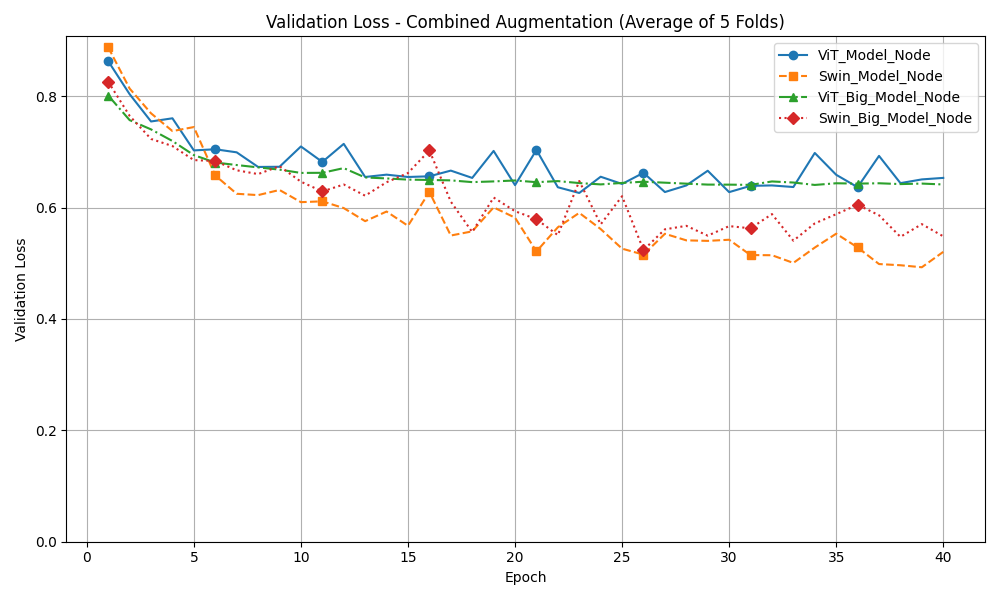
\includegraphics[width=0.9\linewidth]{val_loss_combined_2geo.png}
    \caption{Comparativa del \emph{Validation Loss} a lo largo de las épocas con aumentación combinada (2Geo+2Photo+1SEM).}
    \label{fig:val_loss_combined}
\end{figure}

\subsubsection{Análisis de Sobreajuste en Modelos Swin}

Un fenómeno particular se observó en el escenario de aumentación combinada \texttt{Combined\_2Geo\_2Photo\_1SEM\_x2}, comparando el Swin Standard y el Swin Large. La Figura~\ref{fig:overfitting_analysis} ilustra las curvas de \emph{Training Loss} vs. \emph{Validation Loss} para ambos casos.

\begin{itemize}
    \item \textbf{Swin Standard (Fig.~\ref{fig:swin_std_tv}):} Este modelo muestra un comportamiento clásico de \emph{overfitting} a partir de cierta etapa. El \emph{Training Loss} (línea azul) disminuye drásticamente, convergiendo casi a cero, mientras que el \emph{Validation Loss} (línea naranja) se estabiliza y comienza a divergir ligeramente o estancarse. Esto indica que el modelo, con su capacidad moderada, es capaz de memorizar eficazmente el conjunto de entrenamiento aumentado, pero esta memorización deja de traducirse en mejoras de generalización.
    
    \item \textbf{Swin Large (Fig.~\ref{fig:swin_large_tv}):} En contraste, el modelo grande muestra una dinámica diferente. Su \emph{Training Loss} no disminuye tan abruptamente como en el modelo estándar. Esto es contraintuitivo pero puede explicarse por la dificultad de optimizar una superficie de error mucho más compleja con un dataset limitado. El modelo grande parece "resistirse" más a la memorización rápida, manteniendo una brecha (\emph{gap}) más constante entre entrenamiento y validación. Esto sugiere que, paradójicamente, el modelo más grande podría beneficiarse más de un entrenamiento más prolongado o de un volumen de datos aún mayor para desbloquear su potencial, mientras que el modelo estándar alcanza su techo de rendimiento (y comienza a sobreajustarse) más temprano.
\end{itemize}

\begin{figure}[H]
    \centering
    \subfloat[Swin Standard: Train vs Val]{
        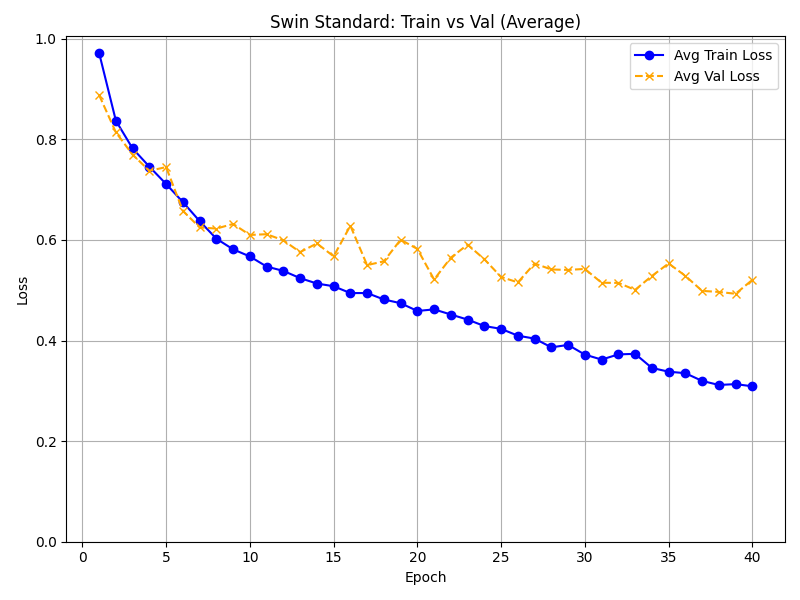
\includegraphics[width=0.9\linewidth]{train_val_swin_std.png}
        \label{fig:swin_std_tv}}
    \\
    \subfloat[Swin Large: Train vs Val]{
        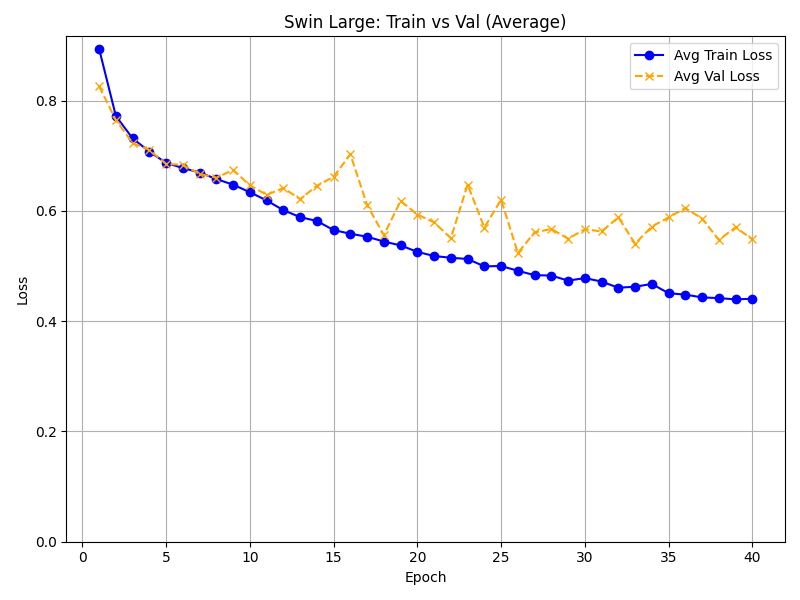
\includegraphics[width=0.9\linewidth]{train_val_swin_large.png}
        \label{fig:swin_large_tv}}
    \caption{Análisis de curvas de entrenamiento y validación bajo aumentación combinada. Se observa un \emph{overfitting} más marcado en la caída del \emph{Training Loss} del modelo estándar en comparación con el modelo grande.}
    \label{fig:overfitting_analysis}
\end{figure}


\subsection{Análisis de Escalabilidad de Datos}

Adicionalmente, se realizó un estudio sobre la influencia del volumen de datos en el rendimiento del modelo, analizando la evolución de la pérdida (loss) mínima alcanzada en validación en función del porcentaje de datos utilizados para el entrenamiento.

La Figura~\ref{fig:loss_vs_data} ilustra esta relación. Se observa una clara tendencia decreciente en la pérdida a medida que aumenta el tamaño del dataset, lo cual confirma que los modelos actuales no han saturado su capacidad de aprendizaje y se beneficiarían significativamente de la incorporación de más muestras etiquetadas. La curva sugiere un comportamiento de rendimientos decrecientes típico, donde las ganancias iniciales al aumentar los datos son rápidas, pero requieren volúmenes exponencialmente mayores para obtener mejoras marginales posteriores.

\begin{figure}[h]
    \centering
    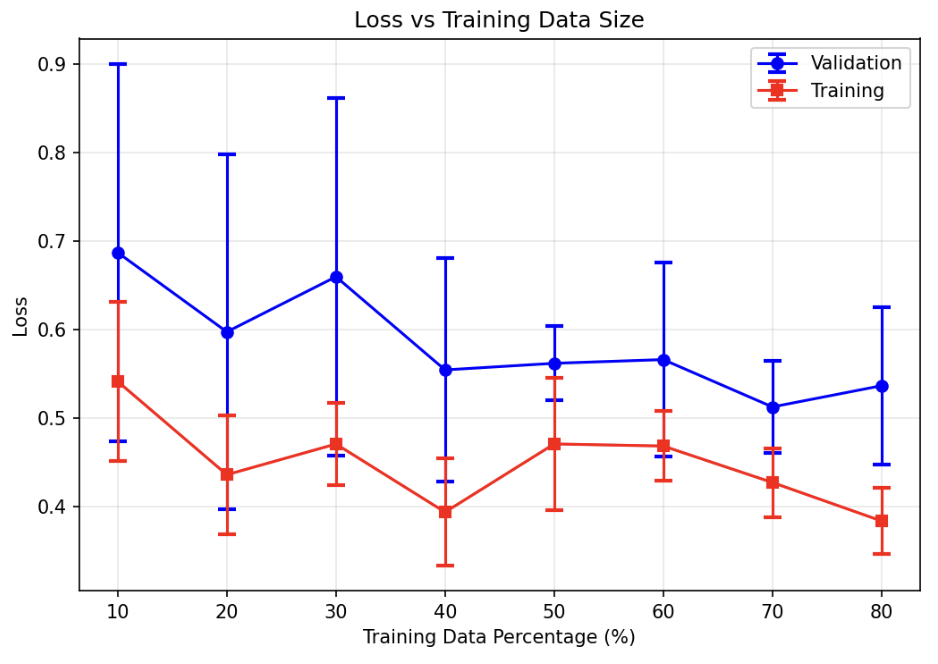
\includegraphics[width=0.9\linewidth]{loss_vs_data_size.png}
    \caption{Relación entre el tamaño del dataset de entrenamiento y la pérdida mínima en validación. La tendencia indica que el aumento en la disponibilidad de datos contribuye consistentemente a la reducción del error del modelo.}
    \label{fig:loss_vs_data}
\end{figure}

\section{Conclusiones}
% - Resumen de hallazgos principales
% - Mejor estrategia de segmentación
% - Limitaciones del trabajo
% - Trabajo futuro

\bibliographystyle{ieeetr}
\bibliography{references}


\end{document}
